\subsection{Spotlights}
In the game, spotlights are used to represent the player's flashlight and the car's head- and tail lights.

Spotlights are modeled in the same way as point lights, with only one exception.
In the case of spotlights, we want to capture the fact that the light forms a cone.
To do that we calculate the \textit{intensity coefficient} given by
\begin{equation*}
    \mathrm{IC} = \frac{\langle l, -d \rangle - R}{r - R},
\end{equation*}
where $d$ is the vector along which the spotlight is directed, and $R$ and $r$ are the parameters defining the light cone \cite{LearnOpenGL-Light-casters}.
The intensity coefficient is then used to multiply each component of the light, giving the result shown in \autoref{fig:spotlights}.
\begin{figure*}[!htb]
    \centering
    \begin{subfigure}[b]{0.475\textwidth}
        \centering
        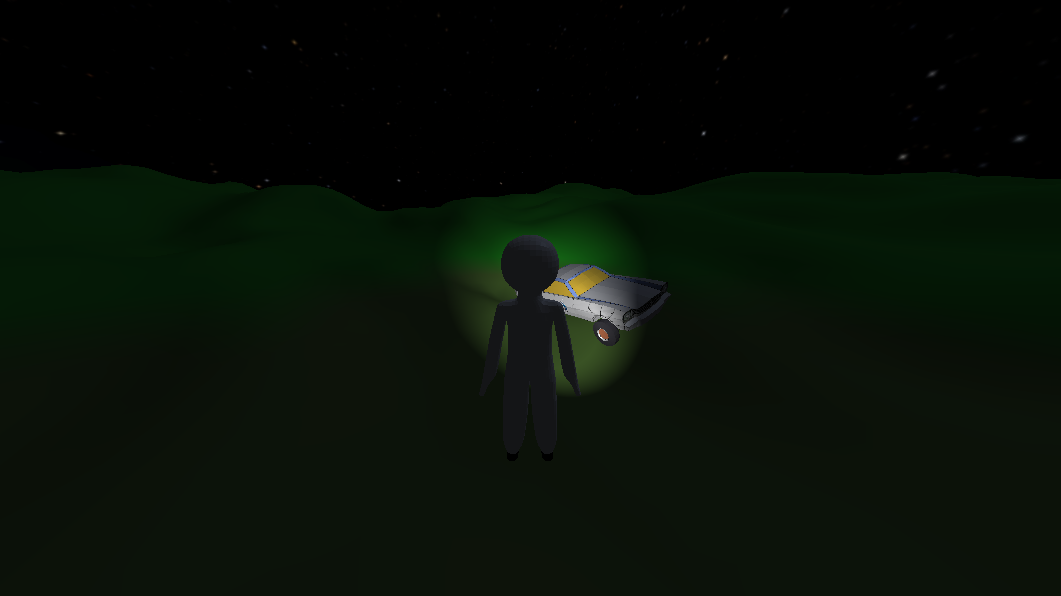
\includegraphics[width=\textwidth]{chapters/theoretical_foundations/sections/lighting/resources/player-flashlight.png}
        \caption[]%
        {{\small Player's flashlight}}
        \label{fig:spotlight-player}
    \end{subfigure}
    \hfill
    \begin{subfigure}[b]{0.475\textwidth}
        \centering
        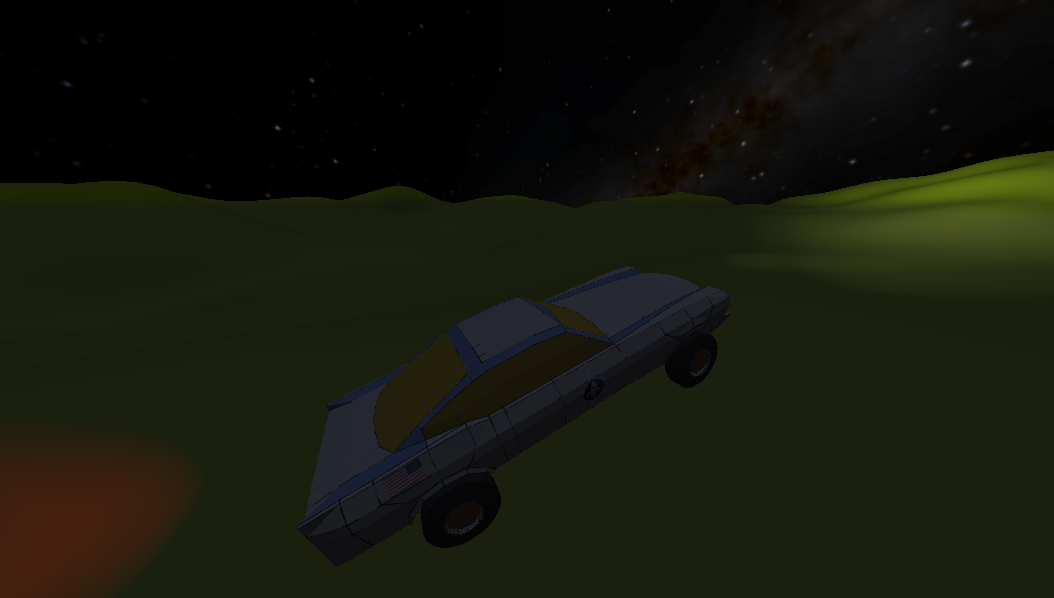
\includegraphics[width=\textwidth]{chapters/theoretical_foundations/sections/lighting/resources/car-lights-spot.png}
        \caption[]%
        {{\small Car illumination}}
        \label{fig:spotlight-car}
    \end{subfigure}
    \caption[]
    {\small Spotlights used in the game}
    \label{fig:spotlights}
\end{figure*}